\documentclass[12pt]{article} 
%\usepackage{times,helvet}
\usepackage{palatino}
%\usepackage[utf8]{inputenc} %useful to type directly diacritic characters
%\usepackage{ssss}
\usepackage{amsmath,amsbsy,amssymb}
\usepackage{sectsty,hangcaption}
%\usepackage{deflist}
\usepackage{fancyhdr}
\usepackage{tabularx}
\usepackage{verbatim}
\usepackage{moreverb}
\usepackage{float,comment}
\usepackage{graphicx}
\usepackage{longtable}
%\usepackage{portland}
\usepackage{booktabs}

\usepackage[super,comma,sort]{natbib} 
\bibpunct[, ]{(}{)}{;}{a}{,}{,}

%must be last package
%\usepackage{hyperref}
\usepackage[debug=false, colorlinks=true, pdfstartview=FitV, linkcolor=blue, citecolor=blue, urlcolor=blue, pdfpagelabels=true]{hyperref}

\textwidth 6.5in
\textheight 9.5in
%\topmargin -.1in
\topmargin -.75in
\newlength{\boxwidth}
\setlength{\boxwidth}{5.8in}
\oddsidemargin -0in
\evensidemargin -0in
\headheight 0.25in

\lhead{{\sl PFLOTRAN Readiness \ldots}}
\chead{\rm - \thepage\ -}
\rhead{\sl\today}
\cfoot{}

\newcommand\flotran{{\sl FloTran}}
\renewcommand{\baselinestretch}{1.0}
\def\EQ#1\EN{\begin{equation}#1\end{equation}}
\def\BA#1\EA{\begin{align}#1\end{align}}
\def\BS#1\ES{\begin{split}#1\end{split}}
%\newcommand{\EQ}{\begin{equation}}
%\newcommand{\EN}{\end{equation}}
\newcommand{\bcr}{\begin{center}}
\newcommand{\ecr}{\end{center}}
\newcommand{\eq}{\ =\ }
\newcommand{\degc}{$^\circ$C}
\renewcommand{\c}{{\rm CO_2}}
\newcommand{\im}{{\rm imb}}
\newcommand{\m}{{\rm mb}}
\newcommand{\ecm}{{\rm ecm}}
\newcommand{\eff}{{\rm eff}}
\newcommand{\eqr}{{\rm le}}
\newcommand{\equ}{{\rm eq}}
\newcommand{\kin}{{\rm kin}}
\newcommand{\rdx}{{\rm rdx}}
\newcommand{\ind}{{\rm id}}
\newcommand{\dep}{{\rm dp}}
\newcommand{\e}{{\rm{e}}}
\newcommand{\erf}{{\rm{erf}}}
\newcommand{\erfc}{{\rm{erfc}}}
\newcommand{\p}{{\partial}}
\newcommand{\A}{{\mathcal A}}
\newcommand{\B}{{\mathcal B}}
\newcommand{\C}{{\mathcal C}}
\newcommand{\D}{{\mathcal D}}
\newcommand{\E}{{\mathcal E}}
\newcommand{\F}{{\mathcal F}}
\newcommand{\G}{{\mathcal G}}
\newcommand{\I}{{\mathcal I}}
\newcommand{\J}{{\mathcal J}}
\newcommand{\M}{{\mathcal M}}
\newcommand{\cO}{{\mathcal O}}
\renewcommand{\P}{{{\mathcal P}}}
\newcommand{\Q}{{\mathcal Q}}
\newcommand{\R}{{{\mathcal R}}}
\renewcommand{\S}{{\mathcal S}}
\newcommand{\T}{{\mathcal T}}
\newcommand{\W}{{\mathcal W}}
\newcommand{\Y}{{\mathcal Y}}
\newcommand{\Z}{{\mathcal Z}}
\newcommand{\rev}{{\rm rev}}
\newcommand{\irr}{{\rm irr}}
\renewcommand{\a}{{\alpha}}
\newcommand{\abar}{{\bar \alpha}}
\renewcommand{\b}{{\beta}}
\renewcommand{\e}{{\epsilon}}
\newcommand{\s}{{\sigma}}
\newcommand{\w}{{\rm H_2O}}
\newcommand{\air}{{\rm N_2}}
\newcommand{\pe}{{\rm Pe}}
\newcommand{\da}{{\rm Da}}
\renewcommand{\k}{{\dot R}^0}
\renewcommand{\L}{\widehat{\mathcal L}}
%\renewcommand{\bar}{\overline}
\newcommand{\dsty}{{\displaystyle}}
\newcommand{\diff}{{\mathcal D}}
\newcommand{\surf}{\equiv \!\!\!}
\newcommand{\bnabla}{\boldsymbol{\nabla}}
\newcommand{\ba}{\boldsymbol{a}}

\newcommand{\balpha}{\boldsymbol{\alpha}}
\newcommand{\bbeta}{\boldsymbol{\beta}}
\newcommand{\bgamma}{\boldsymbol{\gamma}}
\renewcommand{\d}{{\delta}}

\newcommand{\bA}{\boldsymbol{A}}
\newcommand{\bB}{\boldsymbol{B}}
\newcommand{\bb}{\boldsymbol{b}}
\newcommand{\bC}{\boldsymbol{C}}
\newcommand{\bc}{\boldsymbol{c}}
\newcommand{\bcolon}{\boldsymbol{:}}
\newcommand{\bdot}{\boldsymbol{\cdot}}
\newcommand{\bD}{\boldsymbol{D}}
\newcommand{\bE}{\boldsymbol{E}}
\newcommand{\bF}{\boldsymbol{F}}
\newcommand{\bG}{\boldsymbol{G}}
\newcommand{\bg}{\boldsymbol{g}}
\newcommand{\bi}{\boldsymbol{i}}
\newcommand{\bI}{\boldsymbol{I}}
\newcommand{\bJ}{\boldsymbol{J}}
\newcommand{\bK}{\boldsymbol{K}}
\newcommand{\bL}{\boldsymbol{L}}
\newcommand{\bM}{\boldsymbol{M}}
\newcommand{\bn}{\boldsymbol{n}}
\newcommand{\bdelta}{\boldsymbol{\delta}}
\newcommand{\bGamma}{\boldsymbol{\Gamma}}
\newcommand{\bomega}{\boldsymbol{\omega}}
\newcommand{\bOmega}{\boldsymbol{\Omega}}
\newcommand{\bPsi}{\boldsymbol{\Psi}}
\newcommand{\bO}{\boldsymbol{O}}
\newcommand{\bnu}{\boldsymbol{\nu}}
\newcommand{\bdS}{\boldsymbol{dS}}
\newcommand{\bP}{\boldsymbol{P}}
\newcommand{\bq}{\boldsymbol{q}}
\newcommand{\br}{\boldsymbol{r}}
\newcommand{\bR}{\boldsymbol{R}}
\newcommand{\bS}{\boldsymbol{S}}
\newcommand{\bU}{\boldsymbol{U}}
\newcommand{\bu}{\boldsymbol{u}}
\newcommand{\bv}{\boldsymbol{v}}
\newcommand{\bw}{\boldsymbol{w}}
\newcommand{\bx}{\boldsymbol{x}}
\newcommand{\by}{\boldsymbol{y}}
\newcommand{\bY}{\boldsymbol{Y}}
\newcommand{\bz}{\boldsymbol{z}}
\newcommand{\bzero}{\boldsymbol{0}}

\newcommand{\arrows}{~\rightleftharpoons~}
\newcommand{\arrowstab}{\!\!\!\rightleftharpoons\!\!\!}
\newcommand{\longline}{\noindent\rule[-0.1in]{\textwidth}{0.01in}}

\def\water{H$_2$O}
\def\calcium{Ca$^{2+}$}
\def\copper{Cu$^{2+}$}
\def\magnesium{Mg$^{2+}$}
\def\sodium{Na$^+$}
\def\potassium{K$^+$}
\def\uranium{UO$_2^{2+}$}
\def\hion{H$^+$}
\def\bicarbonate{HCO$_3^-$}
\def\cotwo{CO$_2$}
\def\chloride{Cl$^-$}
\def\fluoride{F$^-$}
\def\phosphoricacid{HPO$_4^{2-}$}
\def\nitrate{NO$_3^-$}
\def\sulfate{SO$_4^{2-}$}
\def\souotwooh{$>$SOUO$_2$OH}
\def\sohuotwocothree{$>$SOHUO$_2$CO$_3$}
\def\soh{$>$SOH}

%\renewcommand{\thepage}{\roman{page}}
%\renewcommand{\thepage}{\arabic{page}}
%\renewcommand{\theequation}{\arabic{section}.\arabic{subsection}-\arabic{equation}}
%\renewcommand{\theequation}{\arabic{section}-\arabic{equation}}
%\setcounter{page}{1}

\setlength{\parindent}{0.3125in}
\setlength{\parskip}{2ex plus 0.2ex minus 0.2ex}

\setcounter{secnumdepth}{4}
\setcounter{tocdepth}{4}
\renewcommand{\contentsname}{CONTENTS}

\setlongtables

\pagestyle{fancy}

\thispagestyle{empty}

\begin{document}

{\noindent\bf\Large PFLOTRAN Readiness Applications \hfill \today}

\longline

\noindent
\begin{tabular}{llll}
{\bf Contacts:} &Peter C. Lichtner & 505-667-3420 & lichtner@lanl.gov\\
&Glenn E. Hammond & 509-375-3875 & glenn.hammond@pnl.gov\\
&Bobby Philip & & philipb@ornl.gov
\end{tabular}

\longline

\tableofcontents

\longline

\section{Introduction}

Readiness test for PFLOTRAN consists of several problem sets. 
The first set of problem sets described below applies to a partially saturated groundwater problem with infiltration at the surface with and without transport. A second problem set applies to injection of supercritical CO$_2$ in a deep geologic formation with and without multicomponent reactive transport. The problem sets are briefly described in Table~\ref{tprobset}.

\begin{table}[h]\centering
\caption{Definition of readiness problem sets.}\label{tprobset}
\vspace{3mm}
\begin{tabular}{cl}
\toprule
{\bf Problem Set} & \multicolumn{1}{c}{\bf Description}\\
\midrule
\#1 & Richards mode flow only\\
\#2 & Richards mode coupled to non-reactive transport\\
\#3 & Richards mode coupled to reactive transport\\
\#4 & CO$_2$ mode without transport\\
\#5 & CO$_2$ mode with reactive transport\\
\bottomrule
\end{tabular}
\end{table}

\section{Readiness Application: Problem Set 1}

\subsection{Background}

The Hanford tank farm complex is situated on the Columbia River plateau in a semiarid region in south-central Washington. The site served as a plutonium production facility for nuclear weapons from 1944 to the end of the Cold War era. Storage tanks at the site contain waste fluid streams from the plutonium extraction process. Numerous leaks have occurred at the Hanford Site from single-shelled tanks containing high-level radioactive waste (it has been estimated that 67 out of 149 single-shell tanks have leaked). The largest areas of vadose zone contamination occur in the S-SX Waste Management Area located in the 200 Area of the Hanford site, consisting of the 241-S and 241-SX tank farms, near tanks S-104, SX-108/SX-109, and SX-115. 

\subsection{Problem Description}

The first problem involves solving Richards equation for an isothermal, variably saturated porous medium with infiltration at the top boundary surface. In the Richards formulation the gas pressure is kept constant fixed at atmospheric pressure (101,325 Pa). The porous media is layered consisting of eight homogeneous stratigraphic units from the Hanford 200 Area.

A structured grid is used in the calculation.
A domain size is 80 meters in the vertical. The lateral domain size is determined by the {\tt GRID} keyword through the number of nodes specified by {\tt NXYZ} for {\tt nx} and {\tt ny} and the grid spacing specified by {\tt DXYZ} for {\tt dx} and {\tt dy}. The vertical grid spacing should be fixed at {\tt dz} = 1 meter to accurately determine the boundaries between stratigraphic units. The watertable is located at an elevation of 6 meters from the bottom. 
Either a constant infiltration rate or variable infiltration may be specified at the top boundary. Variable infiltration is read from a file and based on transient rainfall events.
The computational domain is divided into eight stratigraphic units with the material properties listed in Table~\ref{tstrata}.

\begin{table}[h]\centering
\caption{Material properties for each stratigraphic unit taken from \cite{last09} and recently updated (Last private comm.).}\label{tstrata}
\vspace{3mm}
\begin{tabular}{lccccccc}
\toprule
Unit & Elevation [m] & $\varphi$ & $\tau$ [---] & $k$ [m$^2$] & $\a$ [Pa$^{-1}$] & $\lambda$ & $s_r$ [---] \\
\midrule
HD   & 77--80 & 0.262 & 1 & 5.43d-13 & 1.9401d-4 & 0.286 & 0.115 \\ 
H1   & 66--77 & 0.317 & 1 & 9.91d-13 & 3.8801d-4 & 0.486 & 0.110\\
H2   & 51--66 & 0.356 & 1 & 3.34d-14 & 1.0211d-4 & 0.541 & 0.118\\
H3   & 45--51 & 0.398 & 1 & 1.74d-14 & 5.1054d-5 & 0.527 & 0.143\\
CCUz & 41--45 & 0.419 & 1 & 5.06d-14 & 5.1054d-5 & 0.555 & 0.095\\
CCUc & 37--41 & 0.281 & 1 & 7.68d-13 & 1.1232d-4 & 0.425 & 0.192\\
Rtf  & 35--37 & 0.419 & 1 & 5.06d-14 & 5.1054d-5 & 0.555 & 0.095\\
Rwi  & 0--35 & 0.294 & 1 & 9.63d-14 & 1.4295d-4 & 0.402 & 0.139\\
\bottomrule
\end{tabular}
\end{table}

Boundary conditions imposed on the system are specified infiltration at the surface $\bq_0(t)$, fixed pressure at the bottom surface, and no flow conditions at the sides of the domain.

\subsection{Governing Equations}

The governing equation is Richards equation given by
\EQ
\frac{\p}{\p t} \varphi s \rho + \bnabla\cdot\bq\rho \eq Q,
\EN
where $\varphi$ denotes the porosity of the porous medium, liquid saturation is denoted by $s$, $\rho$ designates the molar fluid density taken as pure water, and $Q$ denotes a source/sink term. The Darcy velocity $\bq$ is computed from the expression
$\bq_\a$ denotes the Darcy flow rate defined by
\EQ
\bq \eq -\frac{kk_r}{\mu} \bnabla \big(P-W\rho g \bz\big),
\EN
where $P$ denotes fluid pressure, $k$ refers to the intrinsic permeability, $k_r$ denotes the relative permeability, $\mu$ denotes the fluid viscosity, $W$ denotes the formula weight of water, $g$ denotes the acceleration of gravity, and $z$ designates the vertical of the position vector. 

The relative permeability $k_r$ is computed from the van Genuchten correlation (van Genuchten, 1980) given by
\EQ\label{krl} 
k_{r} \eq \sqrt{s_e} \left\{1-\left[1-s_e^{1/\lambda} \right]^\lambda \right\}^2, 
\EN 
where the effective saturation $s_e$ is defined as
\EQ 
s_e \eq \frac{s - s_r}{1 - s_r}, 
\EN 
where $s_r$ denotes the residual saturation. Note that $k_{r}$ = 0 for saturations below the residual saturation. 
The liquid saturation is related to capillary pressure $P_c$ [Pa] by the expression
\EQ\label{sat}
s_e \eq \left[1+\left( \alpha |P_c| \right)^n \right]^{-\lambda}. 
\EN 
The constants $n$ and $\lambda$ are related by the expressions 
\EQ\label{lambda} 
\lambda \eq 1-\frac{1}{n}, \ \ \ \ \ n \eq \frac{1}{1-\lambda}. 
\EN 
The inverse relation is given by
\EQ
P_c \eq \frac{1}{\alpha} \left[\left(s_e\right)^{-1/\lambda} -1 \right]^{1/n}.
\EN
For $P\!>\!P_{\rm ref}$, $s\!=\!1$ and the porous medium is fully saturated. 
For $P\!<\!P_{\rm ref}$, the capillary pressure is equal to $P_c \!=\! P_{\rm ref} \!-\!P$ and the saturation is calculated from Eqn.\eqref{sat}.

Boundary conditions of type Dirichlet or Neumann can be imposed on the system of specified pressure or flux, respectively.

\subsection{Numerical Implementation}

A fully implicit backward Euler time stepping method is used for Richards mode. Richards equation is discretized spatially using integrated finite volume. The residual equation for a time step $\Delta t$ thus has the form
\EQ
R_{n} \eq \frac{(\varphi s \rho)_n^{t+\Delta t} - (\varphi s \rho)_n^{t}}{\Delta t} V_n + \sum_{n'} q_{nn'}^{t+\Delta t} \rho_{nn'}^{t+\Delta t} A_{nn'} - Q_n^{t+\Delta t} V_n,
\EN
where $V_n$ denotes the volume of the $n$th control volume, and $q_{nn'}$, $\rho_{nn'}$, and $A_{nn'}$ refer to the Darcy flow velocity, density, and interfacial area at the interface between control volumes $n$ and $n'$. Upstream weighting is used to calculate the density $\rho_{nn'}$. The velocity $q_{nn'}$ is obtained from Darcy's law
\EQ
q_{nn'} \eq -\left(\frac{kk_r}{\mu}\right)_{nn'} \left(\frac{P_n - P_{n'} -W\rho g z_{nn'}}{d_n+d_{n'}}\right),
\EN
where $d_n$, $d_{n'}$ refer to the distances from the control volume center to the interface, and $z_{nn'}$ denotes the vertical distance between control volumes $n$ and $n'$. Harmonic averaging is used to calculate $kk_r/\mu$ at the interface.

\subsection{Input Files}

\subsubsection{PFLOTRAN Input File}

The PFLOTRAN input file for this problem is listed below.

\tiny
\verbatiminput{pflotran_1.in}
\normalsize

\subsubsection{SAMRAI Input File}

The associated SAMRAI input file is given by:

\tiny
\verbatiminput{pflotran_amr_1.in}
\normalsize

\section{Readiness Application: Problem Set 2}

\subsection{Problem Description}

This problem involves flow and transport in which transport of a tracer is combined with the flow problem of Problem Set 1. In this problem a tracer is injected at a depth of 15 meters with a flow rate of 0.187 kg/s over a duration of two weeks representing a 60,000 gallon leak from one of the storage tanks at the Hanford tank farm.

\subsection{Governing Equations}

The same equations for flow are used as in Problem Set 1 with the addition of a source term to represent leaking from an underground storage tank. The transport equations are coupled to the flow equations through the flow velocity $\bq$ and saturation $s$. The reactive transport equations have the general form
\EQ\label{rxntp}
\frac{\p}{\p t} \varphi s \Psi_j + \bnabla\cdot\big(\bq \Psi_j - \varphi s D \bnabla \Psi_j\big) \eq Q_j - \sum_m\nu_{jm}I_m - \frac{\p S_j}{\p t}.
\EN
In this equation $D$ denotes the diffusion/dispersion coefficient taken as a constant, $S_j$ represents sorption processes including ion exchange and surface complexation reactions, and $Q_j$ denotes the source term from the leaking tank. The quantity $\Psi_j$ denotes the total concentration of the $j$th primary species defined as
\EQ
\Psi_j \eq C_j + \sum_i\nu_{ji} C_i,
\EN
for primary species concentration $C_j$ and secondary species $C_i$ with
\EQ
C_i \eq \gamma_i^{-1} K_i \prod_j\big(\gamma_j C_j\big)^{\nu_{ji}},
\EN
with activity coefficients $\gamma_j$, $\gamma_i$ and equilibrium constant $K_i$. The coefficients $\nu_{ji}$ refer to the stoichiometric reaction coefficients. The second term on the right-hand side of Eqn.\eqref{rxntp} describes mineral reactions with rate $I_m$ for the $m$th mineral provided by transition state theory
\EQ
I_m \eq -k_m a_m \big(1-K_m Q_m\big) \zeta_m,
\EN
where $k_m$ denotes the kinetic rate constant, $a_m$ refers to the specific surface area, $K_m$ denotes the equilibrium constant and $Q_m$ designates the ion activity product defined by
\EQ
Q_m \eq \prod\big(\gamma_j C_j\big)^{\nu_{jm}}.
\EN
The factor $\zeta_m$ takes on the values 0 or 1 depending on whether the mineral is present or supersaturated
\EQ
\zeta_m \eq \left\{
\begin{array}{ll}
1, & K_m Q_m >0 \ \text{or} \ \varphi_m>0\\
0, & \text{otherwise}
\end{array} \right.,
\EN
where $\varphi_m$ denotes the mineral volume fraction. The change in mineral concentration is provided by the equation
\EQ
\frac{\p\varphi_m}{\p t} \eq \overline V_m I_m,
\EN
with molar volume $\overline V_m$.

For a non-reactive tracer terms containing the mineral and sorption reaction rates on the right-hand side of Eqn.\eqref{rxntp} vanish and $\Psi_j$ is replaced by the tracer concentration $C_j$. The tracer transport equation is coupled to the flow equation through the saturation and Darcy velocity. The flow equation may be solved independently of the transport equation.

\subsection{Numerical Implementation}

Either fully implicit or operator splitting may be used in the reactive transport mode. For operator splitting the fully coupled transport equations are split into non-reactive and reactive components according to
\EQ
\frac{\p}{\p t} \varphi s \Psi_j + \bnabla\cdot\big(\bq \Psi_j - \varphi s D \bnabla \Psi_j\big) \eq Q_j, \ \ \ \ \ \text{(Step 1)},
\EN
followed by
\EQ
\frac{d}{dt} \varphi s \Psi_j \eq - \sum_m\nu_{jm}I_m - \frac{d S_j}{d t} \ \ \ \ \ \ \ \ \ \ \ \ \ \ \ \ \ \ \ \ \ \ (\text{Step 2}).
\EN

\subsection{Input Files}

\subsubsection{PFLOTRAN Input File}

In the PFLOTRAN input file the source region representing a leaking tank is located at an elevation of 65 meters at the center of the domain. For the input file below, the source region occupies four grid cells horizontally. To keep the same injection volume, this would need to be modified if the grid size is changed.

\tiny
\verbatiminput{pflotran_2.in}
\normalsize

\subsubsection{Auxillary PFLOTRAN Input File}

\tiny
\verbatiminput{src.dat}
\normalsize

\subsubsection{SAMRAI Input File}

The associated SAMRAI input file is given by:

\tiny
%\verbatiminput{pflotran_amr_2.in}
\normalsize

\section{Readiness Application: Problem Set 3}

\subsection{Problem Description}

This problem set is derived from Problem Set 2 coupling Richards equation to reactive transport describing a leak from an underground storage tank at the legacy Hanford nuclear waste site. This is a three-dimensional version of the one-dimensional model presented in \cite{lichtner04}. The model includes transport of cesium release from the underground storage tank with ion exchange reactions resulting in its retardation.

\subsection{Numerical Implementation}

Operator splitting will be used to solve the reactive transport equations.

\section{Readiness Application: Problem Set 4}

\subsection{Background}

$\c$ sequestration (capture, separation, and long term storage) in various geologic media including depleted oil reservoirs, saline aquifers, and oceanic sediments is being considered as a possible solution to reduce green house gas emissions. 
Sequestration in subsurface geologic formations containing saline aquifers could provide permanent storage and thereby help mitigate global climate change. 

Injection of supercritical $\c$ into deep underground reservoirs introduces unique computational challenges. At appropriate $p$-$T$ conditions, supercritical $\c$ is buoyant because of its lower density compared to the brine and rises, eventually becoming trapped by a caprock and spreading laterally as it gradually dissolves into the surrounding brine. As the $\c$ dissolves into the brine, however, the brine becomes heavier and begins to sink resulting in density-driven convective instabilities leading in the formation of $\c$-concentrated brine fingers protruding downward. Convective mixing can result in much more rapid dissipation of the supercritical $\c$ plume compared to diffusive processes alone. Also important is the areal extent of the plume, controlled by competition between the rate of spreading of the plume and the rate at which it dissolves into the brine, which can increase accidental release of $\c$ to the surface through abandoned bore holes and faults. 

\subsection{Problem Description}

This problem involves injection of supercritical $\c$ into a deep geologic formation without chemical reactions. The problem domain is $8000\!\times\!8000\!\times\!250$ cubic meters. Supercritical $\c$ is injected at a depth of 50 meters from the top of the domain. A temperature of 50\degc\ is used at the top boundary at a pressure of $200$ MPa.
An example calculation at two different grid resolutions is shown in Figure~\ref{fco2}.


\begin{figure}[t!]\centering
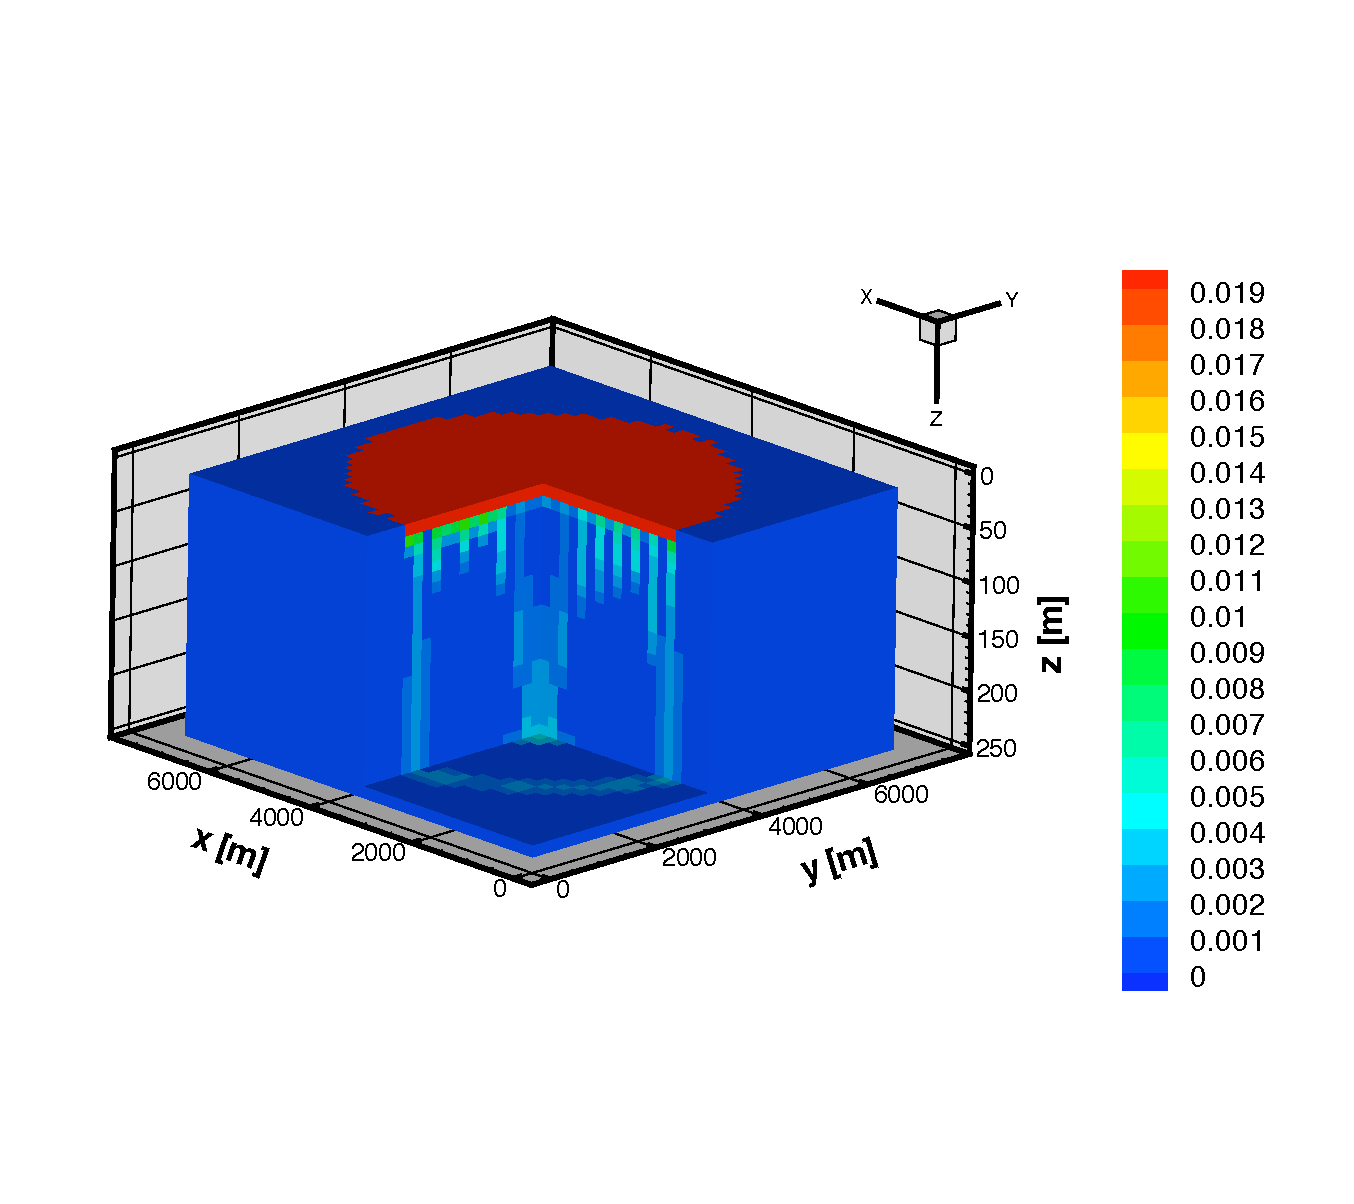
\includegraphics[height=0.325\textheight]{./figs/xl300y-pri-coarse}
  
\vspace{-2.5cm}
  
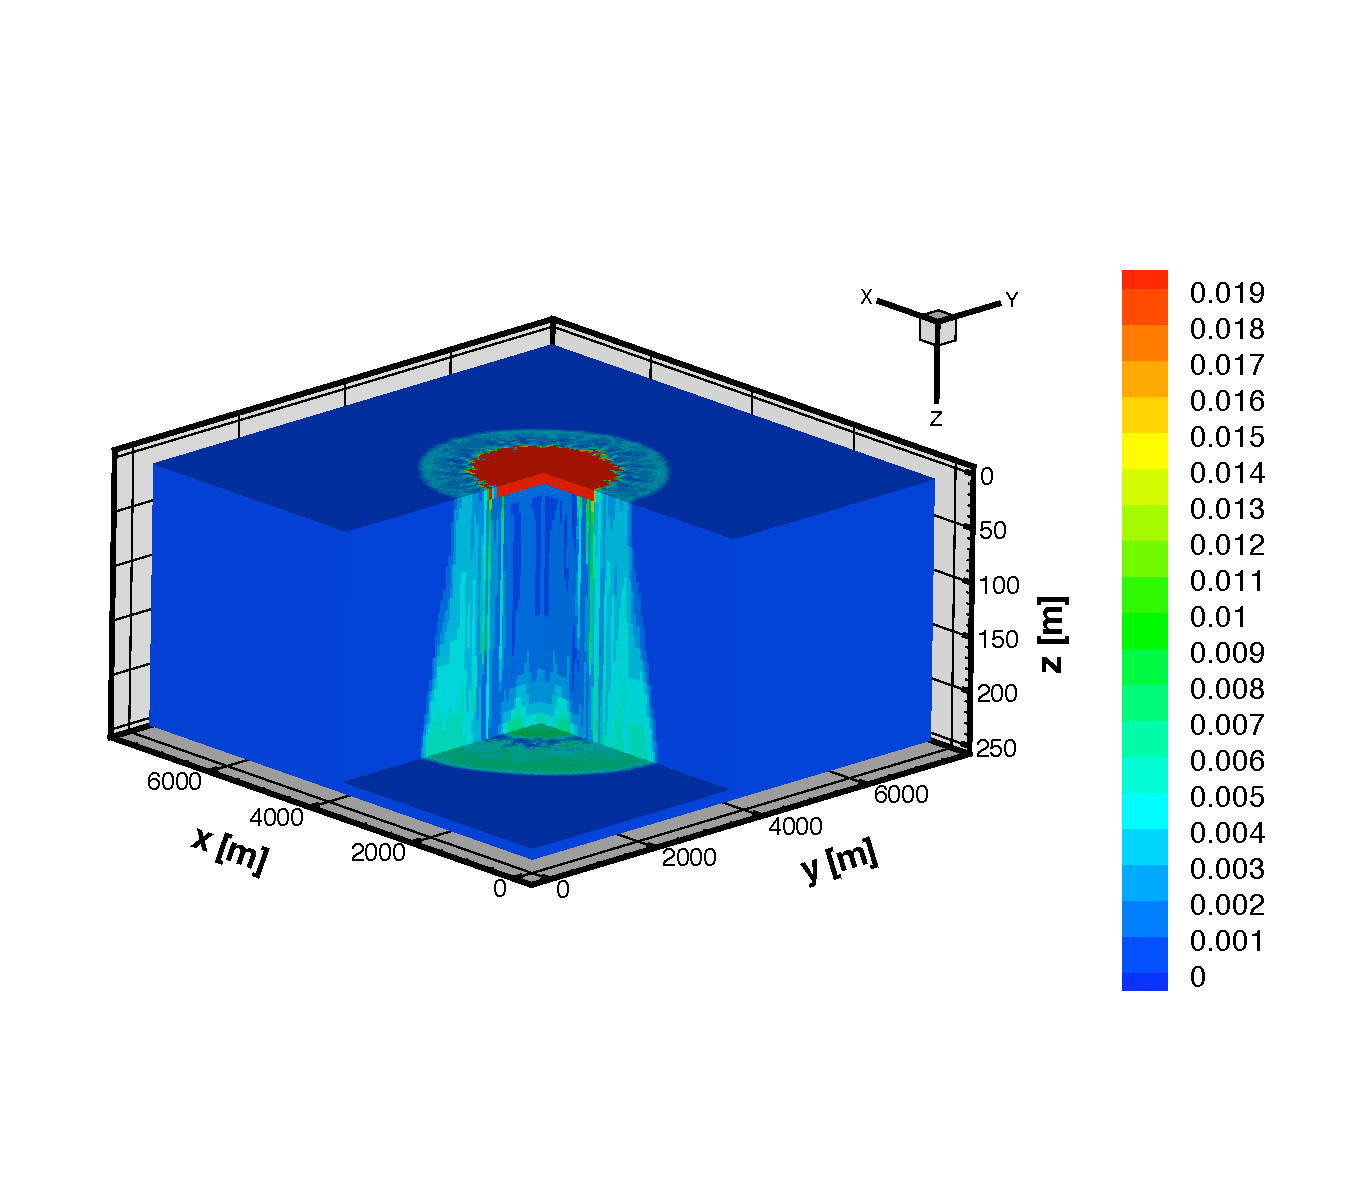
\includegraphics[height=0.325\textheight]{./figs/xl300y-pri-fine} 
  
\vspace{-1.25cm}

\caption{Simulations carried out using PFLOTRAN showing dissolved $\c$ at an elapsed time of 300 years illustrating the dependence of fingering on coarse (top) and fine (lower) grid resolutions \cite{lulich07}. 
The coarse grid consists of $40\!\times\!40\!\times\!25$ nodes with spacing $\Delta x \!=\!\Delta y \!=\! 175$ m and $\Delta z\!=\!10$ m. The fine grid is refined in the $x$ and $y$ directions by a factor 4.
An isotropic permeability of $2\!\times\! 10^{-12}$ m$^2$ is used with a porosity of 15\% typical of sandstone. 
The computational domain is 250 m thick and $7 \!\times\! 7$ km in lateral extent. $\c$ is injected at a rate of 1 Mt/y for 20 years at a depth of 50 m below the top of the domain, corresponding to roughly 75\% of the $\c$ produced by a 1000 MW gas-fired power plant in 20 years. No flow boundary conditions are imposed at the top and bottom and front and back of the domain, and with constant pressure at the left and right sides. 
}\label{fco2}
\end{figure}


\subsection{Governing Equations}

Mass conservation equations employed by PFLOTRAN can be written in the form
\EQ\label{massconv}
\sum_{\a=\w,\,\c} \left\{\frac{\p}{\p t} \big(\varphi s_\a \rho_\a X_i^\a\big) + \bnabla\cdot \big[\bq_\a \rho_\a X_i^\a -\varphi s_\a \rho_\a D_\a \bnabla X_i^\a\big]\right\} \eq Q_i,
\EN
with porosity $\varphi$, molar density $\rho_\a$, diffusivity/dispersivity $D_\a$ and source/sink term $Q_i$. The sum over $\a$ is over all fluid phases present in a particular control volume. In these equations $s_\a$ denotes the volume fraction of phase $\a$ satisfying
\EQ
\sum_\a s_\a \eq 1.
\EN
The mole fraction $X_i^\a$ satisfies the constraint condition
\EQ\label{molefrac}
\sum_i X_i^\a \eq 1.
\EN
The Darcy velocity $\bq_\a$ is given as
\EQ
\bq_\a \eq -\frac{kk_\a}{\mu_\a} \bnabla \Big(P_\a - \rho_\a g z\Big),
\EN
with viscosity $\mu_\a$, acceleration of gravity $g$, and height $z$.

Summing Eqns.\eqref{massconv} over all components $i$ making use of Eqn.\eqref{molefrac} gives
\EQ\label{masstot}
\sum_\a \left\{\frac{\p}{\p t} \big(\varphi s_\a \rho_\a \big) + \bnabla\cdot \big(\bq_\a \rho_\a \big)\right\} \eq Q,
\EN
where
\EQ
Q \eq \sum_i Q_i.
\EN
The equation for $i$ = H$_2$O in Eqn.\eqref{massconv} may be replaced with Eqn.\eqref{masstot}, for example, thereby eliminating the need to consider the diffusion term for H$_2$O.

The energy conservation equation can be written in the form
\EQ
\sum_\a\left\{\frac{\p}{\p t} \big(\varphi s_\a \rho_\a U_\a\big) + \bnabla\cdot\big(\bq_\a \rho_\a H_\a\big) \right\} + \frac{\p}{\p t} \big(\rho_r C_p T \big) - \bnabla\cdot\big(\kappa\bnabla T\big) \eq Q_e,
\EN
as the sum of contributions from each fluid phase and rock,
with internal energy $U_\a$ and enthalpy $H_\a$ of fluid phase $\a$, and rock heat capacity $C_p$ and thermal conductivity $\kappa$. The quantity $Q_e$ denotes the heat source/sink term.

\subsection{Numerical Implementation}

Using a finite volume discretization approach, the governing flow and transport equations are discretized according to
\BA
R_{in}^{k+1} \eq &\sum_\a \left\{\frac{\big(\varphi s_\a \rho_\a X_i^\a\big)_n^{k+1}-(\varphi s_\a \rho_\a X_i^\a)_n^k}{\Delta t} V_n \right. \nonumber\\
&\left. + \sum_{n'} \left[q_{\a,nn'}^{k+1} \rho_{\a,nn'}^{k+1} X_{inn'}^{\a,k+1} -(\varphi s_{\a} \rho_\a D_\a)_{nn'}^{k+1} \frac{X_{i n'}^{\a, k+1}-X_{i n}^{\a,k+1}}{d_{n'}+d_n}\right] A_{nn'}\right\} \nonumber\\
&- Q_i^{k+1} V_n,
\EA
providing the residual function for the $i$th component at the $n$th control volume and $k+1$st time step, where the sum over $n'$ is over all control volumes which connect to the $n$th control volume, $d_n$, $d_{n'}$ refers to the distance for the control volume center to the interface, and $A_{nn'}$ denotes the interfacial area.

The flash method described in the next section is used to solve the governing equations. This approach avoids difficulties encountered with variable switching when used with multilevel solvers.

\subsubsection{Flash Method}

An alternative approach to variable switching is the flash method.
Although the variable switching method is often considered stable and efficient \citep{Pruess99}, it has several shortcomings: 1) it causes perturbations during Newton iterations when phase changes take place; 2) the change in the definition of independent variables affects the structure of the Jacobian matrix; and 3) as a consequence this degrades performance of the preconditioner during the linear solve. Finally, the variable switching approach is not appropriate for use with multilevel solvers because of the possibility for the need to solve for different independent variables on different levels.

In the flash approach the primary variables preserved during the solution of the governing equations. The flash method has been implemented in the FLASH2 mode in PFLOTRAN. The primary variables are $P$, $T$ and the total mole fraction $z_i$ of the $i$th component summed over all phases, defined as:
\BA
z_i &\eq\dfrac{\sum_\a n_i^\a}{\sum_\a \sum_j n^\a_j},\\
&\eq \frac{\sum_\a s_\a \rho_\a x_i^\a}{\sum_{\a} s_\a \rho_\a}.
\EA
Using the expansion
\BA
\frac{n_i^\a}{V} &\eq \frac{n_i^\a}{n_\a}\frac{n_\a}{V_\a}\frac{V_\a}{V_p}\frac{V_p}{V},\\
&\eq \varphi s_\a \rho_\a x_i^\a,
\EA
where where $V$ is the total control volume and $V_p$ denotes the pore volume.
Explicitly for a two-phase ($\a=w$, SC) system where $w$ designates the phase $\w$ and SC designates supercritical $\c$, $z_i$ can be expressed as
\EQ
z_i \eq \frac{s_w \rho_w x_i^w + s_{\rm SC} \rho_{\rm SC} x_i^{\rm SC}}{s_w \rho_w + s_{\rm SC} \rho_{\rm SC}},
\EN
for molar fluid densities $\rho_w$, $\rho_{\rm SC}$ and saturation $s_w$, $s_{\rm SC} \!=\! 1\!-\!s_w$.
The variable $z_i$ is a persistent degree of freedom throughout the simulation.

Introducing $z_i$ into the mass conservation equations gives
\EQ
\sum_\a \left\{\frac{\p}{\p t} \big(\varphi z_i s_\a\rho_\a\big) + \bnabla\cdot \big[\bq_\a \rho_\a x_i^\a -\varphi s_\a \rho_\a D_\a \bnabla x_i^\a\big]\right\} \eq Q_i.
\EN
In this equation $x_i^\a$ is expressed as a nonlinear function of the variables $z_i$. The Jacobian is computed numerically.

Following the notation and formulation found in \cite{nghiem-1985} and \cite{michelsen-1-1982}, let $x_i$, $y_i$ be the mole fraction of component $i$ in liquid and vapor phases, respectively, related by the equilibrium constant $K_i$
\EQ\label{yi}
y_i \eq K_i x_i, 
\EN
and let $\zeta_v$ represent the vapor phase mole fraction defined as
\EQ
\zeta_v\eq\dfrac{\sum_i n_i^v}{\sum_\a \sum_i n^\a_i}.
\EN
Under a phase transformation mass conservation implies the relation
\EQ
z_i \eq \zeta_v y_i + (1-\zeta_v) x_i.
\EN
Using Eqn.\eqref{yi} it follows that
\EQ
z_i \eq \zeta_v K_i x_i + (1-\zeta_v) x_i,
\EN
from which
\begin{subequations}\label{addphase_N2}
\BA
x_i \eq \frac{z_i}{1+(K_i-1)\zeta_v}, 
\EA
and
\BA
y_i \eq \frac{K_i z_i}{1+(K_i-1)\zeta_v}. 
\EA
\end{subequations}
The value of $\zeta_v$ can be found by solving the flash equation (i.e. the Rachford-Rice equation)
\EQ\label{flash}
F(\zeta_v)=\sum_i(y_i-x_i)=\sum_i \frac {z_i(K_i-1)}{1+(K_i-1)\zeta_v} =0.
\EN
Eqn.(\ref{flash}) indicates that the flash method is not able to calculate phase separation for a multiphase system with phase equilibrium distribution coefficients $K_i$ equal to unity, e.g. the water-steam system. Under such situations Eqn.(\ref{flash}) is always satisfied.
 
Since $F(\zeta_v)$ is a monotonically decreasing function of $\zeta_v$, a meaningful solution $0\leq\zeta_v\leq1$ can exist only if 
\begin{subequations}\label{addphase_N3}
\BA\label{liqbc}
\sum_i K_i z_i \geq 1,
\EA
and
\BA\label{vapbc}
\sum_i \frac{z_i}{K_i} \leq 1.
\EA
\end{subequations}
If the equality in Eqn.(\ref{liqbc}) is satisfied the vapor phase is stable, whereas if the equality in Eqn.(\ref{vapbc}) is valid the liquid phase is stable. 
These conditions were referred to by \cite{michelsen-2-1982} in his discussion on phase change calculations. 
It was demonstrated that this criteria is consistent with the tangent plane method applied to the minimization of the Gibbs free energy [\cite{michelsen-1-1982}, \cite{nghiem-1985}]. A more detailed discussion can be found in these references. (In the PFLOTRAN MPHASE mode in which variable switching is employed, the solution of Eqn.(\ref{flash}) for a single node is used as the initial guess for saturation for a phase transition from single to two phase, although the efficiency of this initial guess is not entirely satisfactory because the node does not represent a closed system.)

Eqns.(\ref{addphase_N3}) a, b are used as criteria to determine the existence of a change in phase in the implementation of the flash mode; i.e. if $\sum_i K_i z_i \leq 1$, then only a liquid phase exists; if $\sum_i {z_i}/{K_i} \geq 1$, then only a gas phase exists; otherwise two phases coexist. Once the phase configuration (single aqueous phase, single SC phase, and coexisting two-phase system) is determined, the secondary variables are evaluated in the following steps: 

\noindent
Case 1: single aqueous ($\w$) phase.
The aqueous concentration of the $i$th component is obtained as
\begin{subequations}\label{fla-sec-c1}
\BA
x_i^w = z_i,
\EA
and phase saturations are given by
\BA
s_w = 1, \ s_{SC} =0.
\EA
\end{subequations}

\noindent
Case 2: single supercritical (SC $\c$) phase.
The concentration of the $i$th component in the supercritical phase is obtained as
\begin{subequations}\label{fla-sec-c2}
\BA
x_i^{SC} = z_i,
\EA
and phase saturations are given by
\BA
 s_w = 0, \ s_{SC} =1.
\EA
\end{subequations}
For both cases 1 and 2, the density of either aqueous and SC phase can be obtained from the EOS, since $P$, $T$ and $x_i$ have been determined.

\noindent
Case 3: two phases coexist.
As noted below, the coefficients $K_i$ are not functions of the $\c$ concentration, with their values at given $P$ and $T$ given explicitly by
\begin{subequations}\label{k_value_c}
\BA
K_{\c} =\frac{H_{\c}\gamma_{\c}}{P\phi_{\c}},
\EA
and
\BA
K_{\c} =\frac{P_{\w}^{\rm sat}(T)}{P}.
\EA
\end{subequations}
From these relations the phase composition can be obtained by solving a linear set of equation for the four unknown secondary variables $x_i^\alpha$, ($i$=H$_2$O, CO$_2$) and $\alpha=\w$, SC $\c$. One has
\begin{subequations}\label{k_value_w}
\BA
x_i^{SC} = K_i x_i^w,  \ (i = \w, \ \c),
\EA
subject to the constraints
\BA
{\displaystyle\sum_i} x_i^\alpha=1, \ (\alpha=\w, \ {\rm SC} \ \c).
\EA
\end{subequations}
From these results the phase densities $\rho_\alpha, \alpha=\w$, SC $\c$ can be calculated from $P$, $T$ and $x_i^\alpha$. Once the phase densities are obtained, the saturations $s_\alpha, \alpha=\w$, SC $\c$ can be obtained by solving the linear mass conservation equation
\EQ
\rho_w s_w x_{CO_2}^w + 
\rho_{SC} s_{SC} x_{CO_2}^{SC} = (\rho_w s_w+\rho_{SC} s_{SC}) z_{CO_2},
\EN 
with $s_w=1-s_{SC}$ to give
\EQ
s_{\rm SC} \eq \frac{\rho_{w} (z_{CO_2} - x_{CO_2}^w)}
{\rho_w (z_{CO_2} - x_{CO_2}^w) + \rho_{SC} (x_{CO_2}^{SC} - z_{CO_2})}.
\EN

\subsubsection{Two-Component System}

Currently the FLASH2 mode in PFLOTRAN can only handle systems with two components and two phases, enabling the flash calculation to be carried out in a simplified manner. One important assumption in the implementation in PFLOTRAN is that the activity coefficients in the aqueous phase and the fugacity coefficient in SC phase are not functions of the $\c$ concentration. 
This assumption is consistent with the solubility equations for $\c$ [\cite {garcia01}, \cite{duan2003}, \cite{duan2008}] adapted in PLOTRAN. With this assumption, the phase distribution parameters $K_i(P,\,T)$ are not functions of the mole fractions $z_i, x_i$ and $y_i$, which greatly simplifies the flash calculation. 

For a two-component system the problem may be solved analytically. In this case
\EQ
x_1+x_2\eq 1,
\EN
and
\EQ
K_1 x_1 + K_2 x_2 \eq 1,
\EN
giving
\EQ
x_1 = \frac{1-K_2}{K_1-K_2}, \ \ \ x_2=1-x_1 \eq \frac{K_1-1}{K_1-K_2},
\EN
and
\EQ
y_1 = \frac{K_1(1-K_2)}{K_1-K_2},
\EN
It then follows that
\EQ
\zeta_v \eq \frac{z_i - x_i}{(K_i-1)x_i}, \ (i=1,\,2).
\EN

\section{Readiness Application: Problem Set 5}

This problem involves injection of supercritical $\c$ into a deep geologic formation with chemical reactions between dissolved $\c$ and the formation brine.

\subsection{Problem Description}

In this problem supercritical $\c$ is injected into a sandstone reservoir with carbonate cement in equilibrium with a low concentration brine formation fluid. 

\bibliographystyle{plainnat}
\bibliography{./reference-new}

\end{document}
